
\chapter{Evaluation}\label{ch:evaluation}

We do the evaluation on the hold-out \textit{Clarin-test} dataset,
which has independent speakers and unique transcriptions (Chapter~\nameref{ch:data}).
The architecture of both models is presented in the section~\nameref{sec:synthetic-boosted-model}.
The \textit{Synthetic~Boosted~Model} (the model named~\textit{Boosted} in the table~\ref{table:evaluation})
trained on the entire synthetically augmented dataset achieves more than 12.5\% absolute better the WER score, which equals 14,53\%.
The results on the \textit{Clarin-dev} dataset are comparable.

\begin{table}[h!]
\vspace*{10pt}
\centering
 \begin{tabular}{c c c c c c l}
  \toprule
    WER-test   & CER-test       &  WER-dev       & CER-dev		& Auth.~Audio	& Syn.~Audio	& Model         \\
    \midrule
    16,64       & 3,34              & 16,60	            & 3,39	        & 385		    &               & Base          \\
    14,53       & 2,98              & 14,33	            & 2,78	        & 385	        & 1000	        & Boosted       \\
  \bottomrule
 \end{tabular}
\caption{
The final evaluation results on the \textit{Clarin-test} dataset, and as the reference point
the results on the \textit{Clarin-dev} dataset (Chapter~\nameref{ch:model}).
}
\label{table:evaluation}
\end{table}

In the figure~\ref{fig:synthetic-lm-improvements}, we present two matrices.
On the left is the matrix grouping mistakes of the \textit{Synthetic~Boosted~Model}
by the \textit{Char~Edit~Distance} and the \textit{Word~Edit~Distance}
(as these presented in the section~\ref{sec:conclusions}).
We can see that more than 800 samples have a single spelling mistake.
On the right side, we see the corrected mistakes
with respect to the \textit{Base~Model}.
The most difficult to correct mistakes are on the out of a diagonal, which have
high values of the \textit{Char~Edit~Distance}.
We can observe that the \textit{Synthetic~Language~Model} also corrects mistakes
that have high \textit{Char~Edit~Distance} values.

\begin{figure}[h]
    \centering
    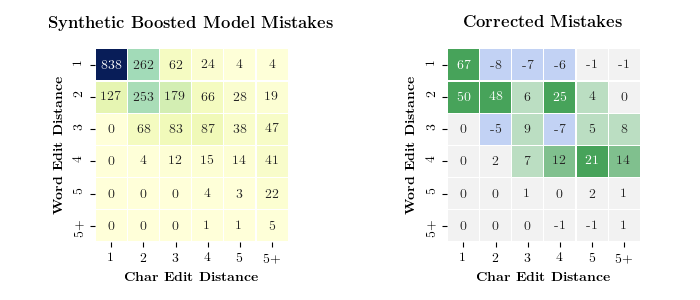
\includegraphics[width=1\textwidth]{figures/evaluation-improvements.png}
    \caption{
On the left, the grouped mistakes of the \textit{Synthetic~Boosted~Model} by
the \textit{Char~Edit~Distance} and the \textit{Word~Edit~Distance}.
On the right, the corrected mistakes, which are defined as the difference between
the \textit{Base~Model} and \textit{Synthetic~Boosted~Model}.
}
\label{fig:evaluation-improvements}
\end{figure}


\subsection*{Error~Analysis}

We do the basic error analysis of the \textit{Synthetic~Boosted~Model}.
At the beginning, we present how the char edit distance (\textit{Levenshtein distance} on the char level)
is distributed among different operations: the \textit{insertion}, the \textit{deletion}, and the \textit{substitution}.
The distribution is presented in the figure~\ref{fig:evaluation-donut}.
The deletion operations are more than two times less than either the insertion or the substitution.
The model tends to predict a char, only while it is confident.

Moreover, inside the donut chart, we mark the share of mistakes caused by the \textit{space} char, where
it should be added or deleted.
Over 15\% of all mistakes are caused by the \textit{space}, which has a high impact on the WER score.
In fact, only a single misspelled space in the sequence composed of four words brings up to 50\% of the WER score.

\begin{figure}[h]
    \centering
    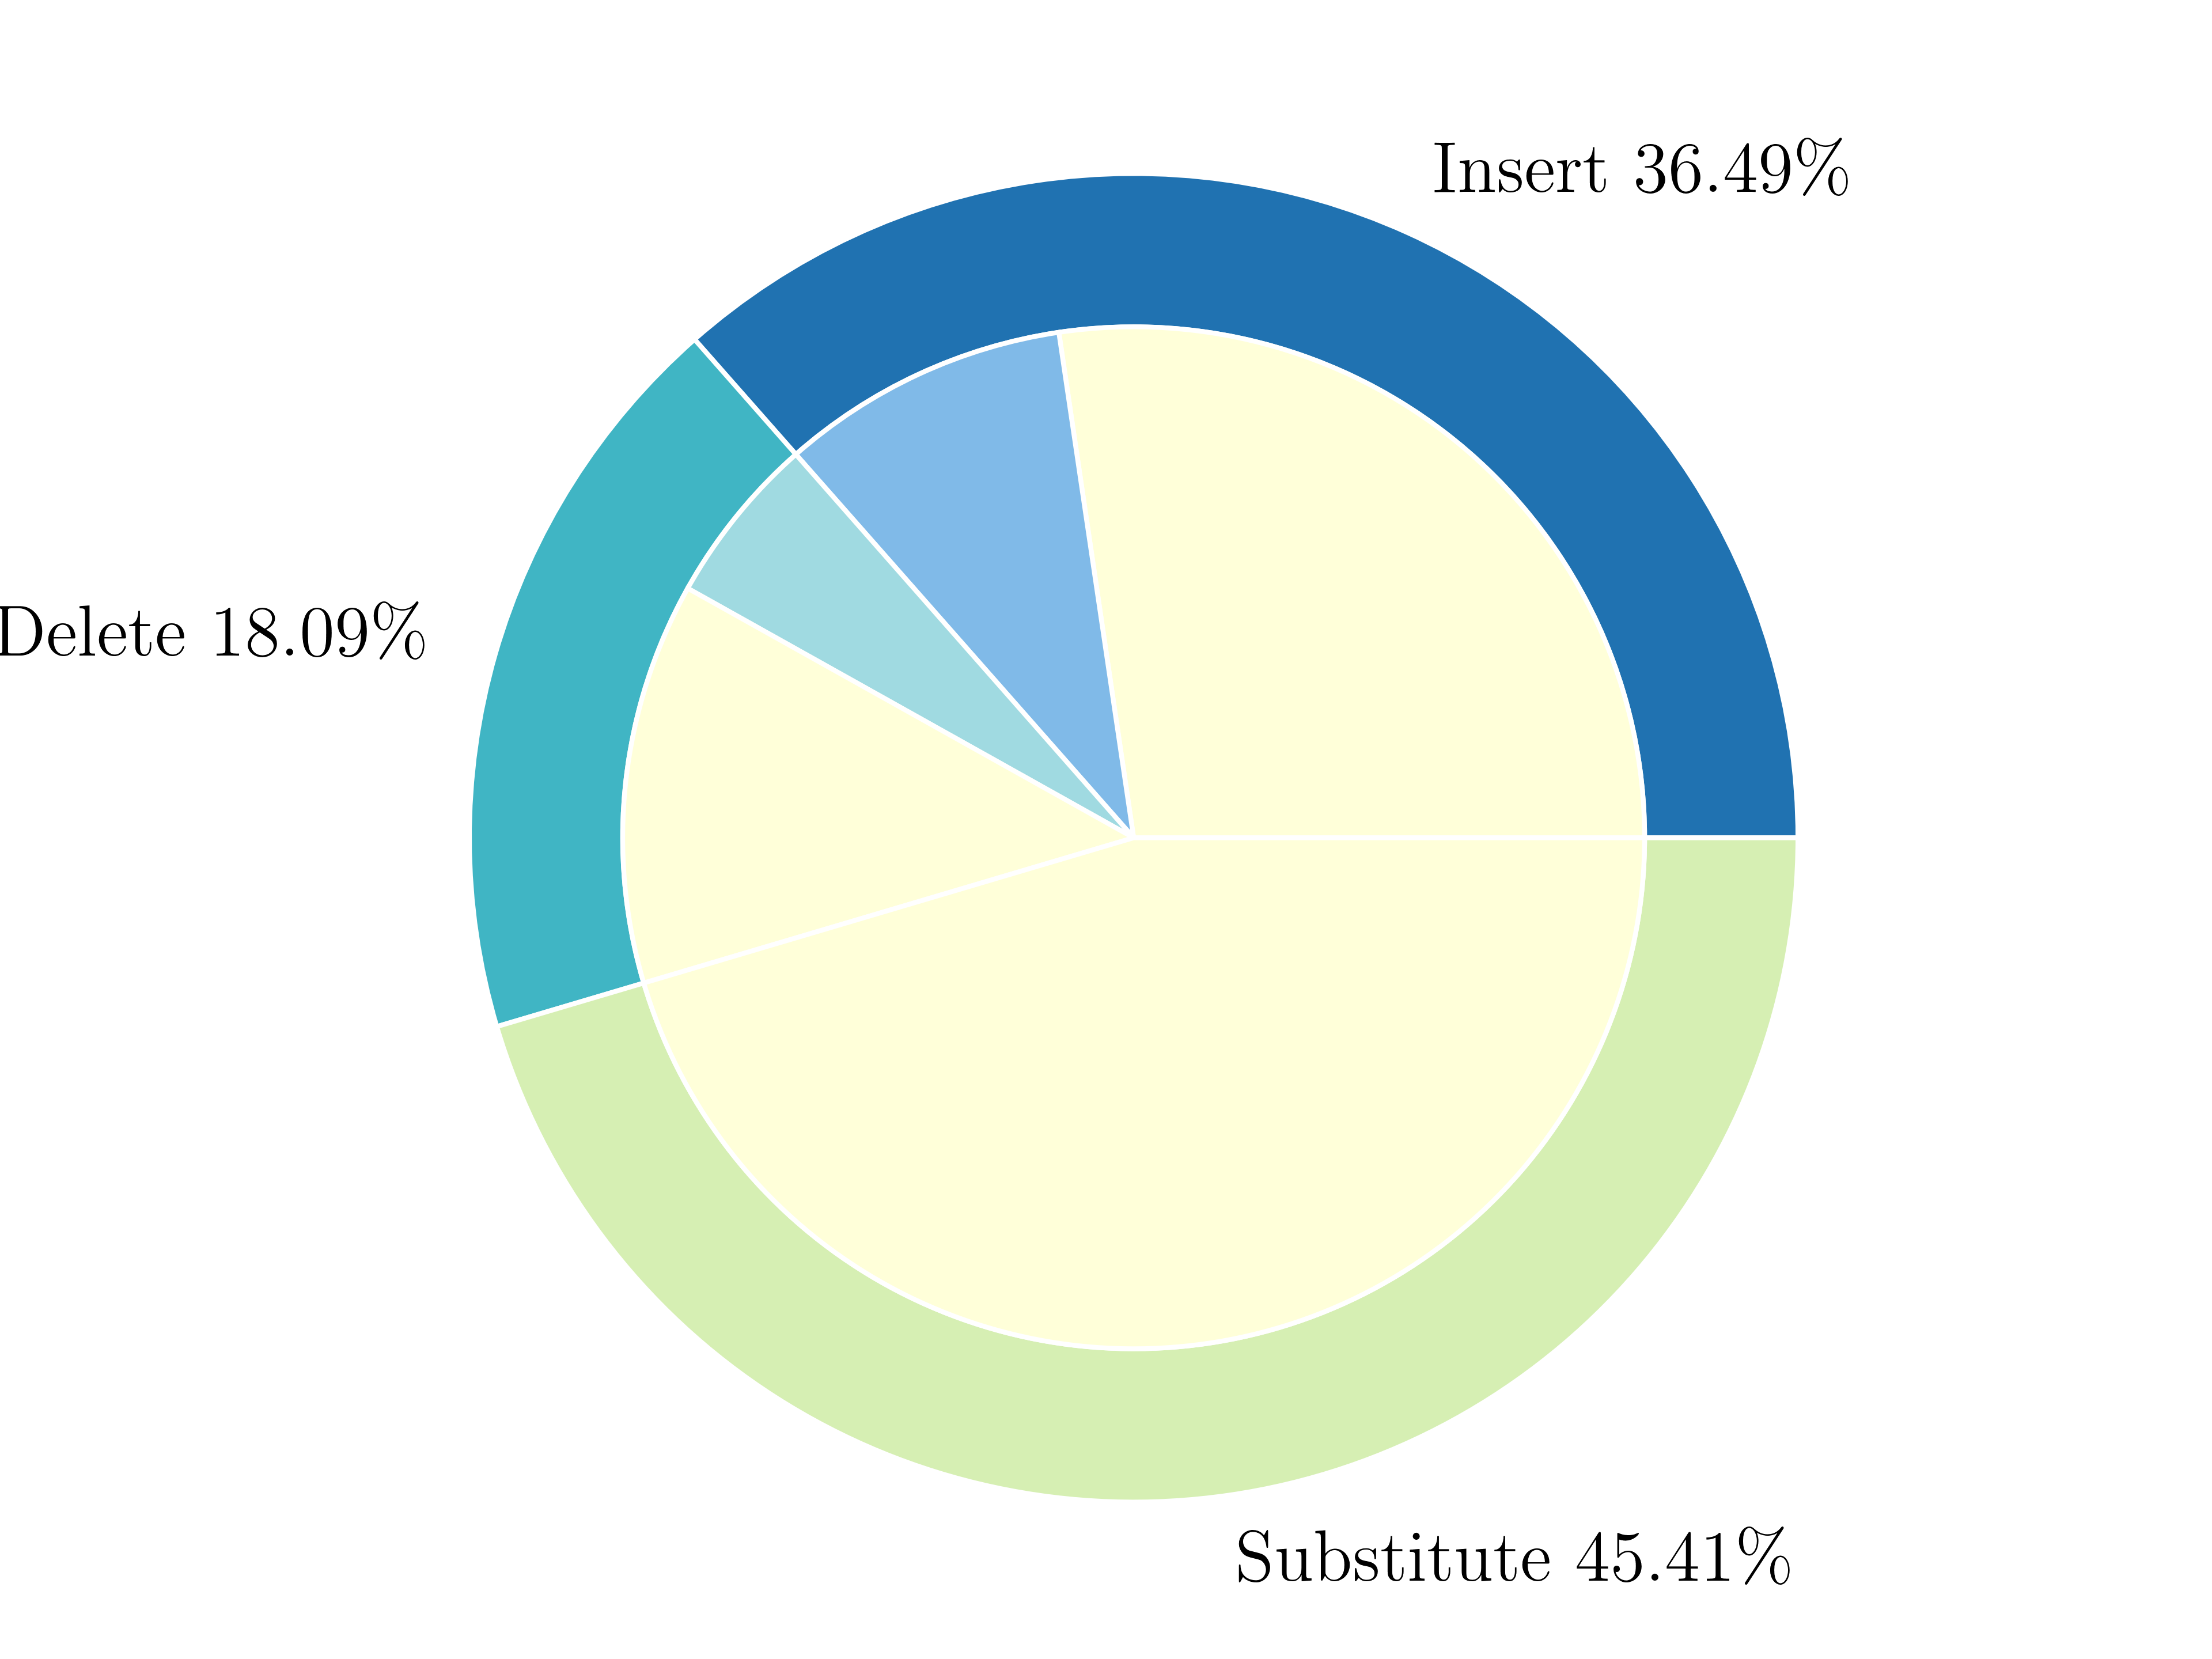
\includegraphics[width=0.45\textwidth]{figures/evaluation-donut.png}
    \caption{
The char edit distance distributed among different operations: the insertion, the deletion, and the substitution.
}
    \label{fig:evaluation-donut}
\end{figure}

The largest group of misspellings is caused by the wrong character prediction, which represents the substitution operation.
To show the mistakes in detail, we present the confusion matrix
in the figure~\ref{fig:evaluation-confusion_matrix}.
The overall pattern is that vowels and consonants are grouped.
There are various concrete patterns which can be easily interpreted.
One of them is that the chars frequently occurred at the end of words~'a',~'e',~'y'
are often each other misspelled.
The letters which sound similar, but depend on the context are written differently, such as
t and d, s and z, or p and b.
Finally, the different grammar rules, for instance, the u and ó, the j and i are hard to be correctly defined.

\begin{figure}[h]
\vspace*{15pt}
    \centering
    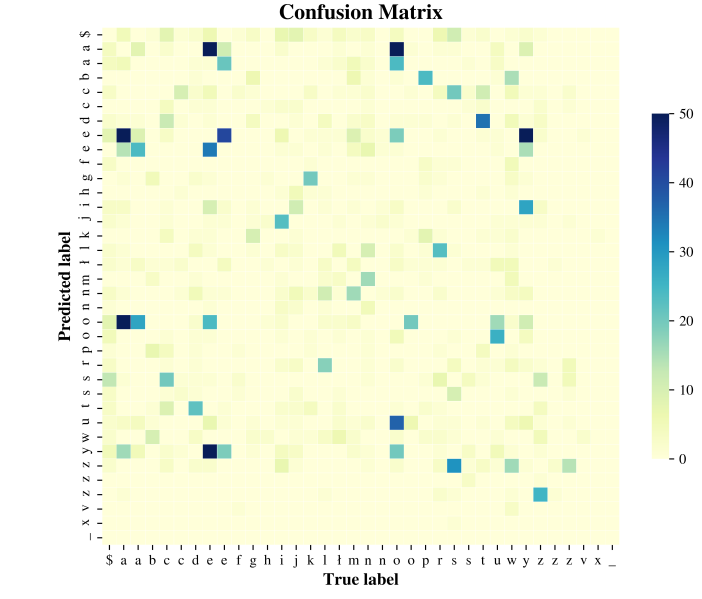
\includegraphics[width=0.8\textwidth]{figures/evaluation-confusion_matrix.png}
    \caption{
The confusion matrix of misspelled characters.
}
    \label{fig:evaluation-confusion_matrix}
\end{figure}
